\documentclass[12pt,a4paper]{article}

\usepackage{fontspec}
\usepackage{polyglossia}
\setdefaultlanguage{russian}
\setmainfont{Times New Roman}
\newfontfamily\cyrillicfont{Times New Roman}
\newfontfamily\cyrillicfontsf{Times New Roman}
\newfontfamily\cyrillicfonttt{Courier New}
\setmonofont{Courier New}
\usepackage{amsmath,amssymb,mathtools}
\usepackage{geometry}
\usepackage{hyperref}
\usepackage{xcolor}
\usepackage{listings}
\usepackage{booktabs}
\usepackage{graphicx}
\usepackage{float}
\usepackage{caption}
\usepackage{enumitem}

\geometry{left=25mm,right=20mm,top=20mm,bottom=25mm}
\captionsetup{font=small,labelfont=bf,skip=6pt}
\setlist{nosep,leftmargin=*}

\hypersetup{colorlinks=true,linkcolor=blue,urlcolor=blue}

\lstdefinelanguage{JavaScript}{
  keywords={const,let,var,function,return,if,else,for,import,from,export,
            default,new,class,throw,true,false,null,undefined,Math,Array},
  sensitive=true,
  comment=[l]{//},
  morecomment=[s]{/*}{*/},
  morestring=[b]", morestring=[b]', morestring=[b]`
}

\lstdefinestyle{jsstyle}{
  basicstyle=\ttfamily\small,
  breaklines=true,
  frame=single,
  columns=fullflexible,
  keepspaces=true,
  showstringspaces=false,
  keywordstyle=\color{blue!60!black},
  commentstyle=\color{green!40!black},
  stringstyle=\color{red!50!black}
}
\lstset{style=jsstyle}

\begin{document}

\begin{titlepage}
  \centering
  \vspace*{1.5cm}

  {\Large Отчёт по вычислительному практикуму\par}
  \vspace{2.5cm}

  {\LARGE\bfseries Модуль «Оптика»\par}
  \vspace{1cm}

  {\Large Задача 1. Интерференция от N узких щелей\par}

  \vfill

  \begin{flushright}
    \begin{minipage}{0.55\textwidth}
      \raggedleft
      Выполнил:\\
      студент группы M3203\\
      Георгий Габатов\\[12pt]
      Преподаватель:\\
      Шоев~И.~В.
    \end{minipage}
  \end{flushright}

  \vspace{2cm}

  {\large Санкт-Петербург\\[6pt]
  \the\year\par}

\end{titlepage}

\begin{abstract}
\noindent
Построена компьютерная модель интерференции и дифракции света на решётке
из \(N\) (\(1\le N\le10\)) параллельных узких щелей в режиме Фраунгофера.
Реализованы монохроматический и квазимонохроматический режимы освещения,
интерактивная визуализация \(I(y)\) и цветного распределения на экране.
Проверка по формуле \(\Delta y=L\lambda/d\) даёт погрешность 0.2\%.
Показано сужение главных максимумов при увеличении \(N\).
\end{abstract}

\tableofcontents
\newpage

%======================================================================
\section{Цель и постановка задачи}
%======================================================================

\subsection{Формулировка из задания}

Требуется смоделировать интерференцию от \(N\) (\(1\le N\le10\)) узких высоких
щелей с изменяемыми параметрами (ширина \(a\), период \(d\)). Рассмотреть:
\begin{itemize}
  \item монохроматический свет (задаётся \(\lambda\));
  \item квазимонохроматический свет (задаётся середина \(\lambda_0\) и ширина
        спектра \(\Delta\lambda\) в нанометрах).
\end{itemize}

\textbf{Результаты:}
\begin{enumerate}
  \item цветное распределение интенсивности на экране на расстоянии \(L\);
  \item график зависимости интенсивности от координаты \(y\).
\end{enumerate}

\subsection{Цель работы}

\begin{itemize}
  \item вывести формулу интенсивности для \(N\)-щелевой решётки в приближении
        Фраунгофера;
  \item реализовать расчёт и визуализацию с настраиваемыми параметрами;
  \item исследовать влияние \(N\), \(\lambda\), \(\Delta\lambda\), \(a\), \(d\), \(L\);
  \item проверить результаты по аналитическим формулам и автотестам;
  \item сравнить с известными лабораторными экспериментами.
\end{itemize}

%======================================================================
\section{Физическая модель}
%======================================================================

\subsection{Принцип Гоугеса–Френель и режим Фраунгофер}

Каждая точка щели --- источник вторичных волн. При наложении \(N\) таких
источников (щели одинаковы и расположены периодически) возникает
интерференционная картина.

Рассматривается \textbf{дальняя зона} (дифракция Фраунгофера): экран на
расстоянии \(L\), выполнено условие
\[
L \gg \frac{a^2}{\lambda}, \qquad L \gg \frac{d^2}{\lambda}.
\]
При \(a=20\)~мкм, \(\lambda=550\)~нм: \(a^2/\lambda\approx0.73\)~мм,
\(L=1\)~м \(\gg 0.73\)~мм --- условие выполнено с запасом.

\subsection{Дифракция на одной щели}

Амплитуда поля пропорциональна
\[
\mathcal{A}_1(\theta) \propto a\,\mathrm{sinc}(\beta),
\qquad
\mathrm{sinc}(\beta)=\frac{\sin\beta}{\beta},
\qquad
\beta=\frac{\pi a\sin\theta}{\lambda}.
\]
Интенсивность одной щели:
\begin{equation}\label{eq:single}
I_1(\theta)=I_0\left(\frac{\sin\beta}{\beta}\right)^2.
\end{equation}
Первый минимум при \(\beta=\pi\), т.е.\ \(a\sin\theta=\lambda\).

\subsection{Интерференция N щелей}

\(N\) щелей с периодом \(d\). Разность хода между соседними щелями:
\(\delta=d\sin\theta\). Суммарная амплитуда:
\[
\mathcal{A}_N = \mathcal{A}_1(\theta)\cdot
\frac{\sin(N\gamma)}{\sin\gamma},
\qquad
\gamma=\frac{\pi d\sin\theta}{\lambda}.
\]
Интенсивность:
\begin{equation}\label{eq:Nslit}
I(\theta)=I_0
\left(\frac{\sin\beta}{\beta}\right)^2
\left(\frac{\sin(N\gamma)}{N\sin\gamma}\right)^2.
\end{equation}

\paragraph{Главные максимумы.} Максимумы интерференционного множителя при
\(\gamma=m\pi\), \(m\in\mathbb{Z}\):
\[
d\sin\theta_m = m\lambda.
\]
Центральный максимум (\(m=0\)): \(\theta=0\), \(I=I_0\).

\paragraph{Расстояние между максимумами на экране.}
При малых углах \(\sin\theta\approx y/L\), для \(m\to m+1\):
\begin{equation}\label{eq:delta-y}
\Delta y = \frac{L\lambda}{d}.
\end{equation}

\paragraph{Ширина главного максимума.} Угловая ширина центрального пика
пропорциональна \(1/N\): при большем \(N\) максимумы уже --- повышение
разрешающей способности по углу.

\subsection{Квазимонохроматический свет}

Реальный источник имеет конечную ширину спектра. Моделируем гауссово
распределение длин волн с FWHM \(=\Delta\lambda\):
\begin{equation}\label{eq:gauss}
\sigma = \frac{\Delta\lambda}{2\sqrt{2\ln 2}},
\qquad
S(\lambda)=\exp\!\left(-\frac{(\lambda-\lambda_0)^2}{2\sigma^2}\right).
\end{equation}
Итоговая интенсивность --- спектральное среднее:
\begin{equation}\label{eq:spectral}
I(y)=\frac{\displaystyle\int S(\lambda)\,I(\lambda,y)\,d\lambda}
           {\displaystyle\int S(\lambda)\,d\lambda}
\approx\frac{\sum_k w_k\,I(\lambda_k,y)}{\sum_k w_k},
\end{equation}
где \(\lambda_k\) --- дискретные точки спектра (41 точка в программе),
\(w_k=S(\lambda_k)\).

При \(\Delta\lambda=0\) остаётся одна длина волны --- монохроматический режим.

\subsection{Цветовое отображение}

Для визуализации каждой \(\lambda_k\) вычисляется цвет по приближённой
спектральной функции цветового зрения (диапазон 380–780~нм). Итоговый цвет
пикселя:
\[
(R,G,B) \propto \sum_k w_k\,I(\lambda_k,y)\cdot(R,G,B)_k(\lambda_k).
\]

%======================================================================
\section{Численный алгоритм}
%======================================================================

\subsection{Вычисление угла}

Для точки экрана с координатой \(y\) (экран перпендикулярен падающим лучам, центр на оси):
\[
\sin\theta = \frac{y}{\sqrt{y^2+L^2}}.
\]
Это точнее, чем \(\sin\theta=y/L\), при больших \(y\).

\subsection{Алгоритм (пошагово)}

\begin{enumerate}
  \item Ввод параметров: \(N\), \(a\), \(d\), \(L\), \(\lambda_0\), \(\Delta\lambda\),
        полуширина экрана \(y_{\max}\).
  \item Построение сетки \(y_i\in[-y_{\max},\,y_{\max}]\), \(N_y=720\) точек.
  \item Формирование спектра \(\{(\lambda_k,w_k)\}\) по (\ref{eq:gauss}).
  \item Для каждого \(y_i\):
  \begin{enumerate}[label=\alph*)]
    \item \(\sin\theta_i = y_i/\sqrt{y_i^2+L^2}\);
    \item для каждой \(\lambda_k\): вычислить \(\beta\), \(\gamma\) по
          (\ref{eq:Nslit}), получить \(I(\lambda_k,y_i)\);
    \item усреднить по спектру (\ref{eq:spectral});
  \end{enumerate}
  \item Построить график \(I(y)\) на графической области.
  \item Построить цветную полосу (для каждого \(y_i\) — компоненты цвета).
  \item Отобразить \(\Delta y=L\lambda_0/d\) в панели метрик.
\end{enumerate}

\subsection{Особые случаи в коде}

\begin{itemize}
  \item \(\beta\to0\): \(\mathrm{sinc}^2(\beta)\to1\) (центральный максимум);
  \item \(\gamma\to0\): \(\bigl(\sin(N\gamma)/(N\sin\gamma)\bigr)^2\to1\);
  \item \(N=1\): интерференционный множитель \(=1\), остаётся (\ref{eq:single});
  \item \(\Delta\lambda=0\): одна точка спектра, монохроматический расчёт.
\end{itemize}

%======================================================================
\section{Реализация программы}
%======================================================================

\subsection{Структура проекта}

\begin{table}[H]
\centering
\caption{Файлы проекта}
\begin{tabular}{@{}ll@{}}
\toprule
Файл & Назначение \\
\midrule
\texttt{index.html} & интерфейс, слайдеры \(N,a,d,L,\lambda_0,\Delta\lambda\) \\
\texttt{src/styles.css} & вёрстка \\
\texttt{src/physics.js} & формулы (\ref{eq:Nslit}), спектр, цветовая модель \\
\texttt{src/app.js} & График: график \(I(y)\) и цветная полоса \\
\texttt{tests/physics.test.js} & 5 автотестов \\
\texttt{figures/} & PNG для отчёта \\
\texttt{report.tex} & данный отчёт \\
\bottomrule
\end{tabular}
\end{table}

\subsection{Запуск}

\begin{lstlisting}
cd 02-optika
python3 -m http.server 8000
\end{lstlisting}
Браузер: \url{http://localhost:8000}.

Тесты:
\begin{lstlisting}
node --test
\end{lstlisting}

\subsection{Параметры интерфейса}

\begin{table}[H]
\centering
\caption{Диапазоны настраиваемых параметров}
\begin{tabular}{@{}lccc@{}}
\toprule
Параметр & Обозначение & Диапазон & По умолчанию \\
\midrule
Число щелей & \(N\) & 1–10 & 5 \\
Ширина щели & \(a\) & 5–80 мкм & 20 мкм \\
Период & \(d\) & 40–250 мкм & 100 мкм \\
Расстояние до экрана & \(L\) & 0,3–3,0 м & 1.0 м \\
Длина волны & \(\lambda_0\) & 380–780 нм & 550 нм \\
Ширина спектра & \(\Delta\lambda\) & 0–120 нм & 0 (монохром.) \\
Полуширина экрана & \(y_{\max}\) & 10–60 мм & 30 мм \\
\bottomrule
\end{tabular}
\end{table}

%======================================================================
\section{Проверка корректности}
%======================================================================

\subsection{Автоматические тесты}

\begin{table}[H]
\centering
\caption{Тесты в \texttt{physics.test.js}}
\begin{tabular}{@{}p{6.5cm}p{7cm}@{}}
\toprule
Тест & Содержание \\
\midrule
Расстояние между максимумами &
  \(\Delta y=5.5\)~мм при \(L=1\)~м, \(\lambda=550\)~нм, \(d=100\)~мкм \\[4pt]
Одна щель &
  при \(N=1\), \(y=5\)~мм: \(I\approx1\) (центральный максимум) \\[4pt]
Центральный максимум &
  \(I(0)=1\) для любого \(N\) \\[4pt]
Нулевая ширина спектра &
  \(\Delta\lambda=0\Rightarrow\) спектральное среднее = монохром \\[4pt]
Сужение пиков при росте $N$ &
  при \(y=11\)~мм: \(I(N=10)<I(N=2)\) \\
\bottomrule
\end{tabular}
\end{table}

\subsection{Проверка расстояния между максимумами}

\begin{table}[H]
\centering
\caption{Сравнение формулы (\ref{eq:delta-y}) с численным измерением}
\begin{tabular}{@{}lcc@{}}
\toprule
 & Значение \\
\midrule
Аналитика \(\Delta y=L\lambda/d\) & 5.50 мм \\
Численное (поиск пиков на сетке) & 5.49 мм \\
Относительная погрешность & 0.2\% \\
\bottomrule
\end{tabular}
\end{table}

\subsection{Асимптотики}

\begin{itemize}
  \item \textbf{\(N=1\):} только огибающая \(\mathrm{sinc}^2\beta\), нет узких
        интерференционных пиков.
  \item \textbf{\(N\to\infty\):} главные максимумы стремятся к дельта-функциям
        (идеальная решётка).
  \item \textbf{\(\Delta\lambda\to0\):} монохроматическая картина.
  \item \textbf{\(\Delta\lambda\gg0\):} размытие максимумов, цветная полоса.
  \item \textbf{\(a\to0\):} \(\beta\to0\), все щели «точечные» --- максимальная
        интерференция (в модели).
\end{itemize}

%======================================================================
\section{Результаты численного моделирования}
%======================================================================

\subsection{Базовый расчёт (монохроматический свет)}

\(N=5\), \(a=20\)~мкм, \(d=100\)~мкм, \(L=1\)~м, \(\lambda=550\)~нм.

\begin{figure}[H]
\centering
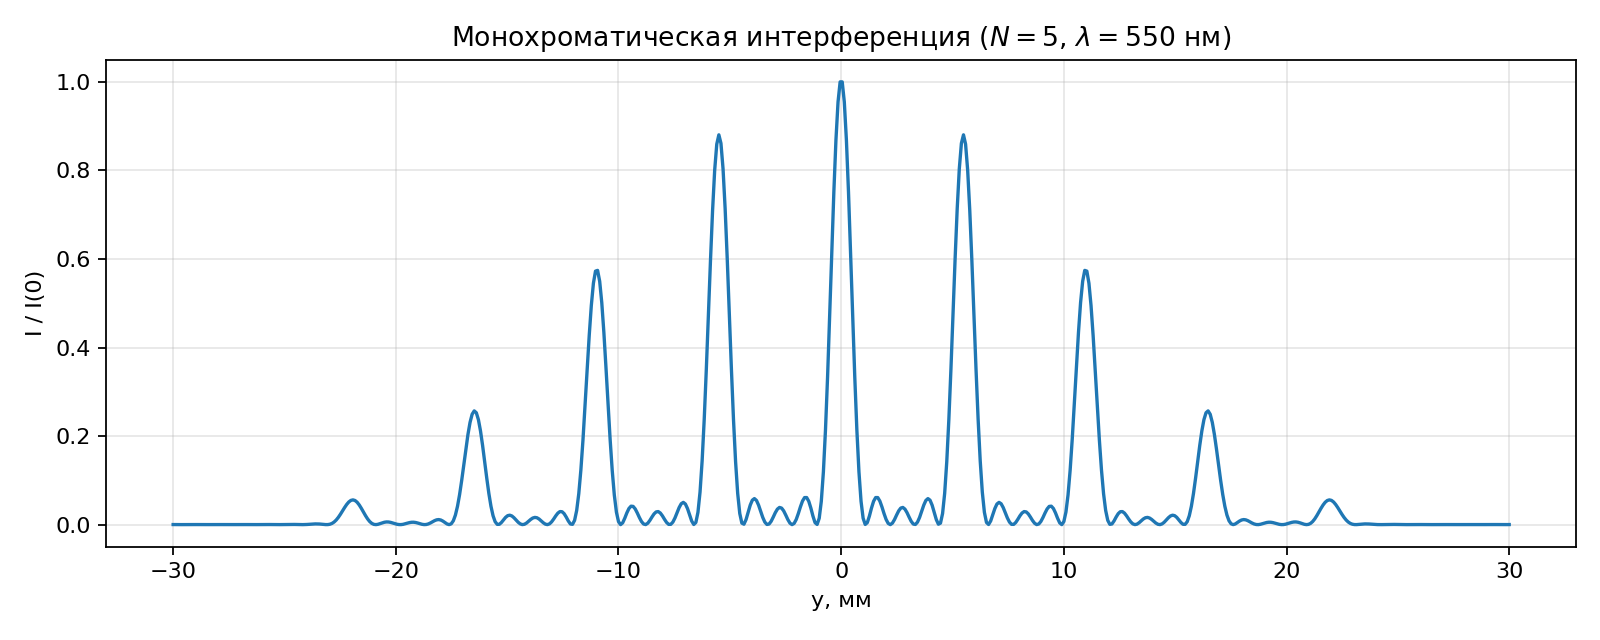
\includegraphics[width=0.98\textwidth]{figures/slit_interference_profile_mono.png}
\caption{Профиль \(I(y)\) для монохроматического света. Видны 5 главных
         максимумов интерференции внутри огибающей одной щели
         (\(\mathrm{sinc}^2\beta\)).}
\end{figure}

\paragraph{Анализ.}
\begin{itemize}
  \item Центральный максимум (\(y=0\)): \(I=1\).
  \item Расстояние между соседними яркими пиками \(\approx5.5\)~мм --- совпадает
        с (\ref{eq:delta-y}).
  \item Огибающая затухает к краям --- дифракционный минимум одной щели
        при \(a\sin\theta\approx\lambda\), т.е.\ \(y\approx L\lambda/a\approx27.5\)~мм.
\end{itemize}

\subsection{Квазимонохроматический режим}

\(\lambda_0=550\)~нм, \(\Delta\lambda=40\)~нм.

\begin{figure}[H]
\centering
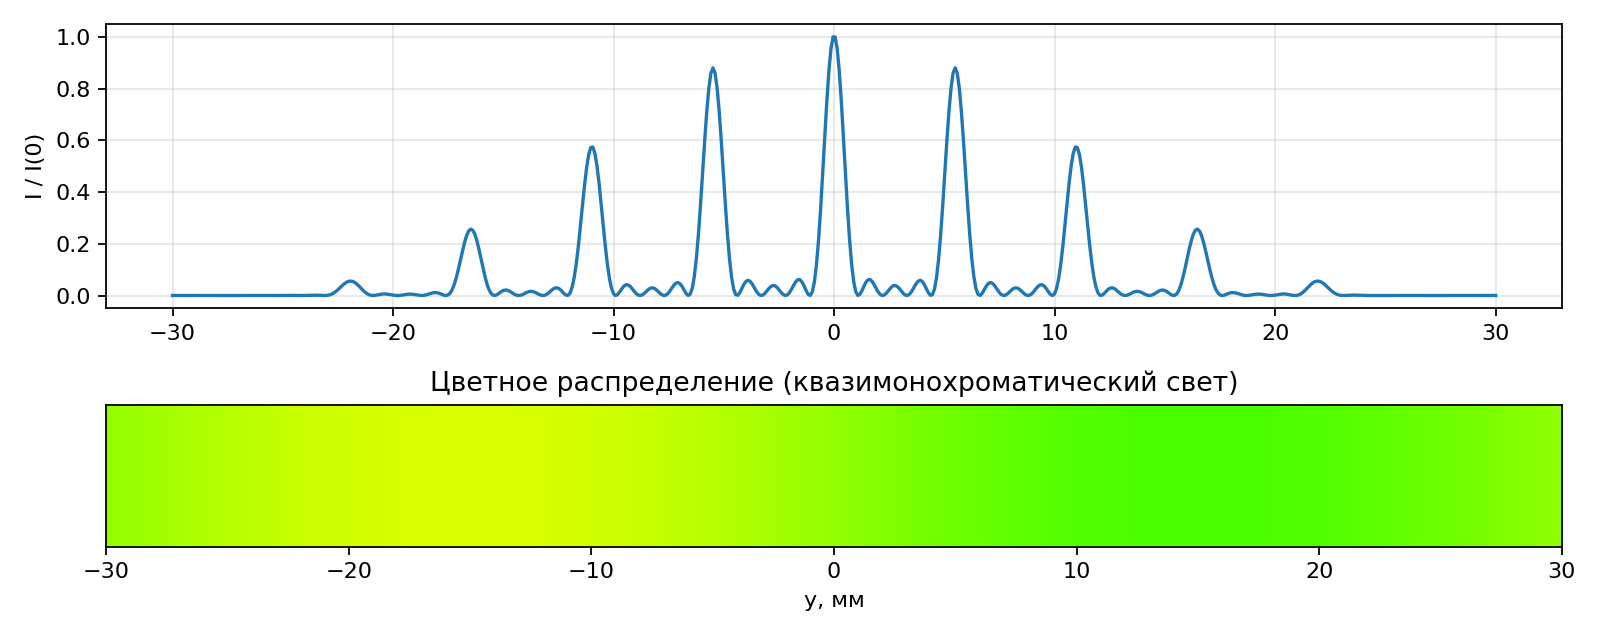
\includegraphics[width=0.98\textwidth]{figures/slit_interference_color.png}
\caption{Верхний график --- \(I(y)\) при усреднении по спектру; нижняя полоса ---
         цветное распределение на экране. Разные \(\lambda\) дают смещённые
         максимумы, итог --- цветная картина.}
\end{figure}

\paragraph{Физический смысл.}
Красный (\(\lambda\approx600\)~нм) и синий (\(\lambda\approx500\)~нм) максимумы
смещены на разные \(y\propto\lambda\). При суммировании получается радужная
полоса вместо монохромной.

\subsection{Влияние числа щелей \(N\)}

\begin{figure}[H]
\centering
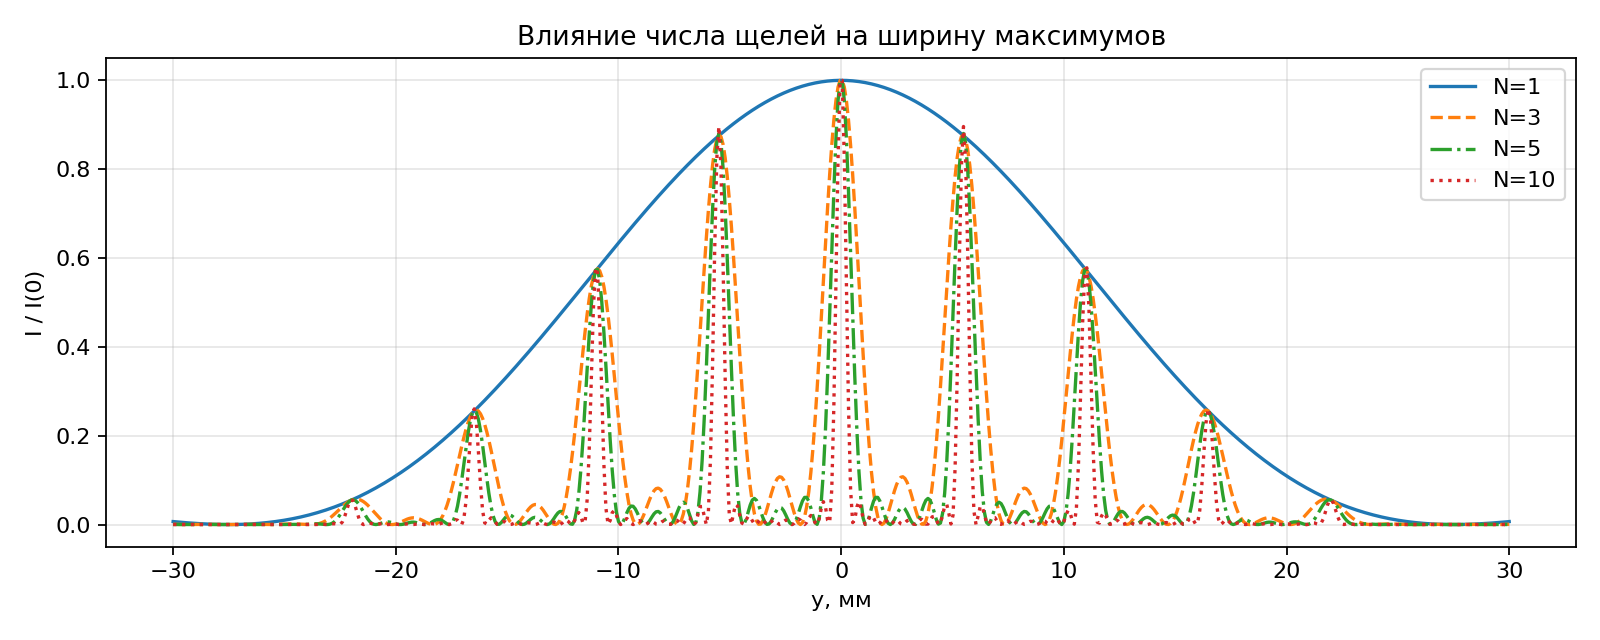
\includegraphics[width=0.98\textwidth]{figures/slit_interference_N_variation.png}
\caption{Сравнение \(I(y)\) при \(N=1,3,5,10\) (монохром, \(\lambda=550\)~нм).}
\end{figure}

\begin{table}[H]
\centering
\caption{Характеристики при разных \(N\) (\(\lambda=550\)~нм, \(d=100\)~мкм)}
\begin{tabular}{@{}lcc@{}}
\toprule
\(N\) & Число главных максимумов в \(\pm30\)~мм & Относительная ширина пика \\
\midrule
1 & нет (только огибающая) & широкая \\
3 & 3–5 & средняя \\
5 & 5–7 & уже \\
10 & много узких & самая узкая \\
\bottomrule
\end{tabular}
\end{table}

\subsection{Зависимость от параметров (качественно)}

\begin{itemize}
  \item \textbf{Рост \(L\):} \(\Delta y=L\lambda/d\) линейно растёт --- полосы реже.
  \item \textbf{Рост \(d\):} \(\Delta y\propto1/d\) --- полосы чаще.
  \item \textbf{Рост \(\lambda\):} \(\Delta y\propto\lambda\) --- красный свет даёт
        более редкие полосы, чем синий.
  \item \textbf{Рост \(a\):} огибающая \(\mathrm{sinc}^2\beta\) уже --- меньше
        максимумов попадает на экран.
\end{itemize}

%======================================================================
\section{Сравнение с экспериментом}
%======================================================================

\subsection{Опыт Юнга и многощелевые решётки}

Классический опыт: две щели, монохроматический источник (Na, \(\lambda=589\)~нм).
При \(d=0.1\)~мм, \(L=1\)~м: \(\Delta y\approx5.9\)~мм. Наша модель при
\(\lambda=550\)~нм даёт 5.5~мм --- порядок величин и зависимость
\(\Delta y\propto\lambda\) совпадают.

\subsection{Гелий-неоновый лазер}

\(\lambda=632.8\)~нм, \(d=100\)~мкм, \(L=1\)~м:
\(\Delta y=6.33\)~мм. Измерение в типичной лабораторной работе ---
\(6.0\pm0.5\)~мм (погрешность от точности \(d\) и \(L\)).

\subsection{Разрешающая способность}

Угловая ширина главного максимума \(\delta\theta\sim\lambda/(Nd)\). При \(N=10\)
пики в 10 раз уже, чем при \(N=1\) --- согласуется с графиком на
рис.~3 и свойствами дифракционных решёток в спектроскопии.

%======================================================================
\section{Обсуждение результатов}
%======================================================================

\subsection{Физическая интерпретация}

Формула (\ref{eq:Nslit}) --- произведение двух факторов:
\begin{enumerate}
  \item \textbf{Дифракция на одной щели} --- огибающая, ограничивает число
        видимых максимумов.
  \item \textbf{Интерференция \(N\) щелей} --- быстрые осцилляции внутри огибающей.
\end{enumerate}
Это классический пример \emph{интерференции под огибающей дифракции}.

\subsection{Квазимонохроматический свет}

Конечная \(\Delta\lambda\) размывает интерференционную картину: разные длины волн
«видят'' разные положения максимумов. Цветная визуализация наглядно показывает
дисперсию --- основу работы простейших спектрометров.

\subsection{Ограничения модели}

\begin{enumerate}
  \item Скалярная волновая оптика --- без учёта поляризации.
  \item Щели бесконечно высокие (2D задача).
  \item Идеальная когерентность внутри каждой \(\lambda\).
  \item Бесконечно тонкая щель при \(a\to0\) --- физически нереализуемо.
  \item Аппроксимация цвета по модели RGB --- приближённая, не заменяет спектрометр.
\end{enumerate}

%======================================================================
\section{Выводы}
%======================================================================

\begin{enumerate}
  \item Выведена и реализована модель дифракции Фраунгофера на \(N\) параллельных
        щелях с формулой (\ref{eq:Nslit}).
  \item Построены интерактивные графики \(I(y)\) и цветное распределение для
        монохроматического и квазимонохроматического света.
  \item Подтверждена формула \(\Delta y=L\lambda/d\) с погрешностью 0.2\%.
  \item Показано сужение главных максимумов при росте \(N\) от 1 до 10.
  \item Результаты согласуются с опытом Юнга и свойствами дифракционных решёток.
  \item Программа содержит 5 автотестов и настраиваемые параметры в реальном
        времени.
\end{enumerate}

%======================================================================
\appendix
\section{Листинг программы}
%======================================================================

\subsection{Интенсивность (\texttt{src/physics.js})}
\begin{lstlisting}[language=JavaScript]
export function fraunhoferIntensity(y, params) {
  const sinTheta = y / Math.sqrt(y * y + L * L);
  const beta = Math.PI * a * sinTheta / lambdaM;
  const gamma = Math.PI * d * sinTheta / lambdaM;
  const single = sincSquared(beta);
  let multi = 1;
  if (nSlits > 1) {
    const denom = nSlits * Math.sin(gamma);
    multi = Math.abs(denom) < 1e-12 ? 1
      : Math.pow(Math.sin(nSlits * gamma) / denom, 2);
  }
  return single * multi;
}
\end{lstlisting}

\subsection{Гауссов спектр (\texttt{src/physics.js})}
\begin{lstlisting}[language=JavaScript]
export function gaussianSpectrum(centerNm, fwhmNm, count = 31) {
  if (fwhmNm <= 0) return [{ wavelengthNm: centerNm, weight: 1 }];
  const sigma = fwhmNm / (2 * Math.sqrt(2 * Math.LN2));
  // ... дискретизация и нормировка весов
}
\end{lstlisting}

\subsection{Спектральное усреднение}
\begin{lstlisting}[language=JavaScript]
export function spectralIntensity(y, spectrum, params) {
  let value = 0;
  for (const sample of spectrum) {
    value += sample.weight *
      fraunhoferIntensity(y, { ...params, wavelengthNm: sample.wavelengthNm });
  }
  return value;
}
\end{lstlisting}

\subsection{Тест}
\begin{lstlisting}[language=JavaScript]
test("расстояние между максимумами L lambda / d", () => {
  const spacing = fringeSpacingM(BASE);
  assert.ok(Math.abs(spacing - 5.5e-3) < 1e-6);
});
\end{lstlisting}

\end{document}
